%\documentclass[sigconf, authordraft]{acmart}
\documentclass[sigconf]{acmart}

\usepackage{algorithm}
\usepackage{algpseudocode}
\usepackage{amsmath}
\usepackage{amssymb}
\usepackage{mathtools}
\usepackage{multirow}
\usepackage{booktabs} % For formal tables
\usepackage[outdir=./]{epstopdf}
\usepackage{graphicx}
\usepackage{listings}
\usepackage{setspace}
\doublespacing
\lstset{
  language=C++,
  basicstyle=\ttfamily\footnotesize,
  showspaces=false,
  showtabs=false,
  tabsize=2,
  frame=single,
}
% Copyright
%\setcopyright{none}
%\setcopyright{acmcopyright}
%\setcopyright{acmlicensed}
\setcopyright{rightsretained}
%\setcopyright{usgov}
%\setcopyright{usgovmixed}
%\setcopyright{cagov}
%\setcopyright{cagovmixed}


% DOI
\acmDOI{10.1145/nnnnnnn.nnnnnnn}

% ISBN
\acmISBN{978-x-xxxx-xxxx-x/YY/MM}

% Conference
\acmConference[GECCO '19]{the Genetic and Evolutionary Computation Conference 2019}{July 13--17, 2019}{Prague, Czech Republic}
\acmYear{2019}
\copyrightyear{2019}

%\acmArticle{4}
\acmPrice{15.00}

% These commands are optional
%\acmBooktitle{Transactions of the ACM Woodstock conference}
%\editor{Jennifer B. Sartor}
%\editor{Theo D'Hondt}
%\editor{Wolfgang De Meuter}


\begin{document}
%\title{Cache-Aware Parallel Particle Swarm Optimization}
\title[Two Simple Tricks for Fast Cache-Aware Parallel PSO]{Two Simple Tricks for Fast Cache-Aware Parallel Particle Swarm Optimization}
%%% The submitted version for review should be ANONYMOUS
\author{Jeff Hajewski}
\orcid{1234-5678-9012}
\affiliation{%
  \institution{University of Iowa\\ Department of Computer Science}
  \city{Iowa City} 
  \state{Iowa} 
  \postcode{52242}
}
\email{jeffrey-hajewski@uiowa.edu}

\author{Suely Oliveira}
\affiliation{%
  \institution{University of Iowa\\ Department of Computer Science}
  \city{Iowa City}
  \state{Iowa} 
  \postcode{52242}
}
\email{suely-oliveira@uiowa.edu}

% The default list of authors is too long for headers.
\renewcommand{\shortauthors}{J. Hajewski et al.}


\begin{abstract}
Particle Swarm Optimization is an example of a trivially parallelizable
algorithm where good performance gains can be seen through the use of a single
OpenMP pragma. Writing an \emph{efficient} parallel PSO algorithm, on the other hand, is much more
challenging because although the particle updates can occur independently, they
rely on a shared global state (the global best particle). The difficulty of
maintaining this global state can be seen in the large body of work studying the
parallelization of PSO -- almost uniformly these algorithms rely on a global
synchronization step, which results in idle cores and reduced parallel
efficiency. In this work, we introduce two techniques for implementing a fast and
efficient parallel PSO algorithm: batching the creation of the random weights
and reducing critical section contention via a relaxed consistency guarantee.
Our technique shows impressive performance improvements over prior work, seeing
more than 60\% speed-up over naive parallelization and more than 10\% speed-up
over the cache-aware algorithm. This speed comes at a cost; while our method
quickly reaches an approximate solution, it struggles in environments requiring
a high level of resolution.
\end{abstract}

%
% The code below should be generated by the tool at
% http://dl.acm.org/ccs.cfm
% Please copy and paste the code instead of the example below. 
%
\begin{CCSXML}
<ccs2012>
<concept>
<concept_id>10010147.10010169.10010170.10010171</concept_id>
<concept_desc>Computing methodologies~Shared memory algorithms</concept_desc>
<concept_significance>500</concept_significance>
</concept>
<concept>
<concept_id>10010147.10010178</concept_id>
<concept_desc>Computing methodologies~Artificial intelligence</concept_desc>
<concept_significance>500</concept_significance>
</concept>
<concept>
<concept_id>10010147.10010341.10010349.10010355</concept_id>
<concept_desc>Computing methodologies~Agent / discrete models</concept_desc>
<concept_significance>300</concept_significance>
</concept>
</ccs2012>
\end{CCSXML}

\ccsdesc[500]{Computing methodologies~Shared memory algorithms}
\ccsdesc[500]{Computing methodologies~Artificial intelligence}
\ccsdesc[300]{Computing methodologies~Agent / discrete models}

\keywords{Particle Swarm Optimization, cache-aware algorithms, artificial intelligence}


\maketitle

\section{Introduction}
Particle Swarm Optimization (PSO) \cite{pso} is a global optimization technique
inspired by swarms found in nature (e.g., a flock of birds).
Each particle in the swarm moves in a partially stochastically weighted
combination of two vectors: one in the direction of the best location the
particle has seen locally and one in the direction of the best location seen by
the swarm globally. Here the term ``best'' is with respect to a fitness
function, which is specified in the problem definition.
The swarm maintains a global best position (the position
with the optimal fitness value) and the goal is for this global best position to
converge to the global minimum (maximum) of the nonlinear function being
optimized.  The challenge comes in the form of required compute power -- due to
the curse of dimensionality, a high-dimensional problem requires a large number
of particles. While improved hardware performance can
improve runtime performance, we have found that efficient algorithm
design coupled with efficient implementation can make similar, if not improved
gains in performance. In the authors'
personal experience, making a heap allocation in the wrong spot or even
something as simple as generating a random number in the wrong location can
increase the runtime of a simulation $1000\times$.\\
The contributions of this work are:

\begin{enumerate}
\item An improved cache-efficient algorithm for parallel PSO. In our
  experiments, this improved algorithm obtains $N\times$ speed-ups over the
  naive parallelization of the cache-efficient algorithm introduce in
  \cite{cache-pso}.
\item A technique for reducing critical section contention in OpenMP

\end{enumerate}

While there is a large body of work on parallel PSO using various threading
techniques and GPGPU programming, the goal of our work is to provide a set
of techniques, tools, and modifications to the standard cache-efficient PSO
algorithm that are simple to understand and use.
The average PSO implementor
likely does not have the specialized knowledge requried to write an efficient
CUDA implementation or to implement efficient management and coordination of
threads. Rather than provide a highly specialized implementation, we focus on
simplicity and clarity while still improving performance. For parallelism, we
utilize OpenMP. We leave the distributed implementation for future work.

The organization of the paper is as follows. In Section \ref{sec:pso} we give a
breif overview of PSO, followed by an overview of cache-aware algorithms and the
challenges encountered in parallel algorithms in Section \ref{sec:cache}. We
present our updated PSO algorithm and implementation guidelines in section
\ref{sec:algo} followed by experimental results in Section \ref{sec:results}.

\section{Particle Swarm Optimization}\label{sec:pso}
Particle Swarm Optimization can be simplified into the update of two formulas:
one for a particle's velocity and the other for the particle's position. Define
$\textbf{pbest}$ as the position corresponding to the best seen fitness value
for a given particle (i.e., the local best), $\textbf{gbest}$ as the position
corresponding to the the best seen fitness value globally, and $\textbf{p}$ as
the current position of the given particle. The update formula for velocity is
given by equation (\ref{eq:velocity} and Table \ref{tab:constants} describes
the interpretation of the constants.

\begin{align}
  \textbf{v}_i(t+1) = \omega \textbf{v}_i (t) & +
                                                c_1 \textbf{r}_1\odot (\textbf{pbest}_i(t) -
                                                \textbf{p}_i(t))
  \\\label{eq:velocity}
  &+ c_2 \textbf{r}_2 \odot(\textbf{gbest}_i(t) - \textbf{p}_i(t))\nonumber
\end{align}

Where $\odot$ is the Haddamard product
Once the velocity is computed, the position update is given by equation
(\ref{eq:position}).

\begin{equation}\label{eq:position}
  \textbf{p}_i(t+1) = \textbf{p}_i(t) + \textbf{v}_i(t)
\end{equation}

\begin{table}
  \caption{Description of the velocity update constants.}\label{tab:constants}
  \begin{tabular}{ll}\toprule
  \textbf{Constant} & \textbf{Description}\\\midrule
  $\omega$ & Momentum\\
  $c_1$ & Explore towards local best\\
  $c_2$ & Exploration towards global best\\
  $r_1$ and $r_2$ & sampled from $U(0,1)$\\\bottomrule
  \end{tabular}
\end{table}

Algorithm \ref{alg:pso} describes the basic PSO algorithm.

\begin{algorithm}
  \caption{Basic PSO algorithm.}\label{alg:pso}
  \begin{algorithmic}[1]
    \Procedure{PSO}{N}
    \State $\texttt{particles} \gets \texttt{initialize}(N)$
    \Repeat
    \For{$\textbf{p} \in \texttt{particles}$}
    \State \texttt{p.UpdateVelocity(\textbf{gbest})}
    \State \texttt{p.UpdatePosition()}
    \EndFor
    \Until Convergence
    \EndProcedure
  \end{algorithmic}
\end{algorithm}

Particles are initialized randomly within the bounds of the search space
$[\texttt{x\_min}, \texttt{x\_max}]$. Some implementations also set a random
intiail velocity for each particle; however, we found it simpler and equally
effective to initialize all particles with zero velocity. In our initial
experiements, we found improved convergence by reflecting particles off the
boundary of a predefined search space using $[x_{\min}, x_{\max}]$. The
reflection was performed by negating the velocity component and offsetting the
particle from the boundary by the amount it would have exceeded the boundary for
the respective position component.
However, we decided to use an open search space with no boundary to give a more
pessimistic view of our algorithm.

Our implementation allows for a predefined minimum and maximum value for
components of the velocity vector -- in practice these should be no greater than
the diameter of the search space.

\section{Prior Work}
There is a large body of work studying the parallelization of PSO. This work can
be broadly broken up into two categories: OpenMP/MPI based methodoligies and
GPGPU based methodoligies (typically via CUDA). OpenMP is a set of pragmas used
with C/C++ or Fortran that automates much of the multi-threading process. MPI
(Message Passing Interface) is a library used for communicating between processes.
The advantage of the OpenMP/MPI
approach is flexibility in parallelization due to the difference in
architecture. GPGPU approaches are more restricted due to the GPU architecture
-- branching in work groups in a GPU can dramatically reduce performance. The
primary challenge in parallelizing PSO is efficiently updating \texttt{gbest}.

The most common approach to parallelizing PSO is through the use of
sub-swarms. Each sub-swarm is assigned to a thread and sub-swarms share the
sub-swarm best amongst other swarms as a way to communicate
\textbf{gbest}. Many \cite{cooppso, comppso, optionpso}
build the sub-swarm implementation with OpenMP and MPI. Peng et
al. \cite{multicore-pso} also investigate the sub-swarm approach to
parallelization but explore several different swarm communication topoligies and
use Java threading rather than OpenMP and MPI. All works achieve similar linear
speed-ups at low thread counts ($<20$ threads).

The other common approach to parallelizing PSO is via GPGPU programming. The
challenge with GPGPU programming is two-fold: minimizing communication between
the GPU and CPU, which is costly, and avoiding branching within the GPU
kernel\footnote{a kernel in GPGPU programming is the name of the procedure being
  run on  the GPU}. When grouped threads (referred to as a warp) within a GPU
start to diverge due to branching, the
GPU executes one branch at a time.
This can be difficult to avoid in the PSO algorithm where a core part
of the aglorithm is finding the globally optimal particle (i.e., \texttt{gbest}.
To get around this,
some work \cite{gpu-ppso, gpu-pso} uses the GPU primarily for evaluating the
fitness function across all particles simultaneously.
Others, such as Calazan et al. \cite{swarmgrid}, perform the entirety of
the PSO algorithm on the GPU, transferring data from the CPU to the GPU at the
beginning of the algorithm and then transferring the data back to the CPU from
the GPU at the end of the algorithm.
CONTINUE \cite{biopsogpu, multiswarmpso-gpu}

Other recent work \cite{mrcpso, mprso, coop-pso, intrusion-pso} has
studied the use of the MapReduce framework \cite{mapreduce} in parallelizing PSO
for various applications. In most experiments, these works see near linear
scaling with number of nodes added in the MapReduce cluster.
The MapReduce implementations serve as a complementary
approach to the CPU and GPU-based work. For example, each node in the MapReduce
cluster can run an OpenMP and/or
GPGPU-based algorithm. Improvements to the CPU and GPU PSO algorithms directly
flow into the work of the MapReduce-based algorithms. A similar approach of using
MapReduce for coarse-grain parallelism and resiliency while allowing
models to manage the fine-grained
parallelism is also being investigated by the deep learning community \cite{mrpnn,
  heterospark, dlspark}. 

\section{Cache-aware Design}\label{sec:cache}
Modern x86\_64 CPUs typically have three tiers of cache: L1, L2, and
L3. L1 cache is the fastest but has the smallest amount of storage. The caches
decrease in speed and increase in storage as one descends the cache
hierarchy (with L3 being the lowest). When data is to be loaded into a register
the firstCPU first checks the
cache, then RAM, and lastly disk. Rather than load a single piece of data from
RAM into cache, CPUs load a cache line, which is typically 64B. A standard cache
line corresponds to 16 32-bit numbers or 8 64-bit numbers. A cache-aware
algorithm utilizes this information by grouping data such that data utilized by
the algorithm in temporal proximity is physically stored together. This
is referred to as data locality. In other words, we want to keep data that is
accessed at around the same time as close together as possible. Doing so reduces
access to RAM and disk, both of which are substantially more
costly than accessing cache.

\subsection{Data-Oriented Design}
We can use the idea of data locality to
influence the design of our programs. This is one aspect of what is known as
data-oriented design and
is a very common technique in the video game industry, which is known for
writing performance code.
Data-oriented design
differs from object-oriented design in that data is grouped based on access
paterns rather than logical patterns.

\begin{figure}
  \lstinputlisting{../code/particle.cpp}
  \caption{Example of a Particle class using object-oriented
    design.}\label{fig:particle}
\end{figure}

Figure \ref{fig:particle} shows a typical object-oriented implementation of PSO would be to store the
particles in a vector, where each entry of the vector is the particle object of
a specific particle. When a particle gets loaded into cache from memory the
cache line will contain three \texttt{T*}\footnote{\texttt{T} is either a float
  (32 bits) or a double (64 bits)} pointers, the three constant values
$c_1$, $c_2$, and $\omega$, and three function pointers to the fitness,
position, and velocity update functions.

Figure \ref{fig:particles} shows an example of one possible data-oriented design
approach. The key aspects with this design is that particle positions are stored
in a vector, particle velocities are stored in a vector, and particle best
positions are stored in a vector. Rather than encapsulate particle specific
information in a particle object, we place that information in a vector along
with similar information of other particles. The advantage is data
locality. When we update the velocity of one particle, we will be updating the
velocity of other particles. For example, loading the first velocity vector (we
can think of this is a \texttt{T*} pointer for simplicity), the next seven
velocity pointers will also be pulled into cache because they are on the same
cache line. Compare this with the object-oriented approach where we would need
seven different loads from main memory to get these pointers since each particle
object took up an entire cache line.
\begin{figure}
  \lstinputlisting{../code/particles.cpp}
  \caption{Example of a data-oriented design modeling all particles in a PSO
    simulation.}\label{fig:particles}
\end{figure}

\begin{algorithm}
  \caption{Cache-aware algorithm for PSO.}\label{alg:pso-cache}
  \begin{algorithmic}[1]
    \Procedure{PSO-DO}{N}
    \State $\texttt{vel} \gets \texttt{initialize}(N)$ \Comment{velocity vectors}
    \State $\texttt{pos} \gets \texttt{initialize}(N)$ \Comment{position vectors}
    \State $\texttt{bpos} \gets \texttt{pos}$ \Comment{best position vectors}

    \Repeat
    \State $\texttt{gbest} = \text{argmin}_{\texttt{pos}}\texttt{fitness}(p)$
    \For{$(i, v) \in \texttt{enumerate}(\texttt{vel})$}
    \State $\texttt{local} \gets (\texttt{pos}[i] -
    \texttt{bpos}[i])$
    \State $\texttt{global} \gets  (\texttt{pos}[i]
    - \texttt{gbest})$
    \State $v \gets \omega v + c_1 r_1 \texttt{local}  + c_2 r_2 \texttt{global}$
    \EndFor
    \For{$(p, v) \in \texttt{zip}(\texttt{pos}, \texttt{vel})$}
    \State p += v
    \EndFor
    \Until convergence
    \EndProcedure
  \end{algorithmic}
\end{algorithm}

\section{Cache-aware Parallel PSO}\label{sec:algo}
We make several improvements to the framework for cache-efficient PSO proposed
in \cite{cache-pso}. While none of these improvements is a major structural
change to the algorithm of PSO or the data-oriented design, we found that the
net effect was a dramatic improvement in performance.

\paragraph{Random Weights} One of the major speed-ups we achieved was through
the generation of the random weights $r_1$ and $r_2$. The original description of
PSO \cite{pso} has two calls to \texttt{rand()} during the velocity update for each
component of the velocity vector. We surveyed a number of highly cited works in
PSO literature \cite{pso-development, pso-overview, pso-tutorial} and found in
all descriptions of the algorithm the random values $r_1$ and $r_2$ are sampled
for each element of $\textbf{v}$ (i.e., for $\textbf{v}\in\mathbf{R}^n$ there
are $n$ unique values of $r_1$ and $n$ unique values for $r_2$). We modify this
approach to use a single value $r_1$ and a single value for $r_2$ for all
components of \textbf{v}. Additionally, in the effecient implementation we batch
the generation of these values each time the velocities are updated.
There are two advantages to this approach: we can keep
these random values in cache and we avoid expensive calls to random number
generation routines. This can be seen in Figures \ref{fig:naive-par} and
\ref{fig:efficient-par} -- the naive approach makes two calls to
\texttt{random\_uniform} for each particle. On the other hand, the efficient
approach indexes the $r$-value vectors \texttt{r1s} and \texttt{r2s}, which are
created at the start of each call to \texttt{UpdateVelocity}. Some readers may
note that this is a rather obvious optimization -- we agree. However, in
practice it seems it is an optimization that is frequently overlooked.
Another potential criticism of this approach is that it reduces variation in the
updated velocity, which could potentially slow convergence. In our experience,
the speed-up gained by using a single $r_1$ and $r_2$ outweighs any slowed
convergence resulting from reduced diversity.

\paragraph{Reducing Critical Section Contention} Updating \texttt{gbest}
requires checking all particles against the current \texttt{gbest} and updating
when a position with a better fitness value is found. This is a classic
reduction scenario, which can be done in $O(\lg n)$ time. OpenMP provides the
facilities to handle this efficiently, but only for a few simple types and
operations. Unforutnately, these do include \texttt{std::vector<T>}. To get
around this we do a linear scan of all particles in parallel. This presents its
own challenge due to the data race that occurs when multiple threads attempt to
update \texttt{gbest}. Figure \ref{fig:naive-update} shows an example of a
standard use of OpenMP's \texttt{critical} section to avoid the data race. This
reduces performance because the critical section is hit for every particle on
every update. Inspired by the work on distributed deep learning [CITE], where
they perform asynchronous updates in a manner such that distributed workers are
not guaranteed to have the latest information, we use two nested if-statements
with the \texttt{criticle} section on the inner statement, as shown in Figure
\ref{fig:efficient-update}. The intuition behind this is quite simple -- rather
than take a hit on the \texttt{critical} section for every single particle, we
have all particles first check if they could possibly be the best global
partical by checking against the current \texttt{gbest}. If this fails, they
miss the critical section and move on. In the even the first check passes, the
particle then hits the \texttt{critical} section. As demonstrated in our
experiements, this produced a substantial speed-up. However, this does not come
for free -- those familiar with asynchronous, distributed deep learning
algorithms will note that while these systems improve overall performance, they
do so at the cost of a reduced rate of convergence. Similar to the prior section
on the random weights, the convergence of the swarm is reduced, but the overall
runtime performance is increased.

\begin{figure}
  \lstinputlisting{../code/efficient_update.cpp}
  \caption{Efficient update in a critical section for the efficient parallel PSO
    algorithm.}
  \label{fig:efficient-update}
\end{figure}

\begin{figure}
  \lstinputlisting{../code/naive_update.cpp}
  \caption{Naive update in a critical section for the naive parallel PSO
    algorithm.}
  \label{fig:naive-update}
\end{figure}

\paragraph{Auto-vectorization}
The difference between Figure \ref{fig:naive-par} and Figure
\ref{fig:efficient-par} is pulling the inner loop into a separate function. This
allows the compiler to more easily optimize that piece of code by making the
relationship between the different vectors clear -- there is no pointer aliasing
between \texttt{i} values. In our experiments, for simple loops like this it is
difficult to beat the compiler by hand-writing AVX instructions, especially
without domain expertise in writing efficient, low-level code.

\begin{algorithm}
  \caption{Cache-aware parallel PSO}\label{alg:par-pso}
  \begin{algorithmic}[1]
    \Procedure{Parallel-PSO}{N}
    \State $\texttt{n\_threads} \gets \texttt{getn\_hardware\_threads}()$
    \State $\texttt{tp} \gets \texttt{ThreadPool}()$
    \State $\texttt{vel} \gets \texttt{initialize}(N)$
    \State $\texttt{pos} \gets \texttt{initialize}(N)$
    \State $\texttt{bpos} \gets \texttt{pos}$

    \State $n = N/\texttt{n\_threads}$ \Comment{Assume $N \mod
      \texttt{n\_threads} = 0$}
    \For{$(i, t) \in \texttt{enumerate}(\texttt{tp})$}
    \State $vs \gets \texttt{vel}[ni:n(i+1)]$
    \State $ps \gets \texttt{pos}[ni:n(i+1)]$
    \State $bps \gets \texttt{bpos}[ni:n(i+1)]$
    \State $\texttt{t(Run}(vs, ps, bps))$
    \EndFor
    \For{$t \in \texttt{tp}$}
    \State \texttt{t.join()}
    \EndFor
    \EndProcedure
  \end{algorithmic}
  \begin{algorithmic}[1]
    \Procedure{Run}{\texttt{vs}, \texttt{ps}, \texttt{bps}}
    \State $n \gets \texttt{ps.size()}$
    \Repeat
    \For{$i = 1 \to n$}
    \State $\texttt{gbest} \gets \min\{\texttt{gbest}, \texttt{po}$
    \EndFor
    \For{$i = 1 \to n$}
    \State 
    \EndFor
    \Until convergence
    \EndProcedure
  \end{algorithmic}
\end{algorithm}

\begin{figure}
  \lstinputlisting{../code/naive_par.cpp}
  \caption{Naive loop parallelization with OpenMP.}\label{fig:naive-par}
\end{figure}

\begin{figure}
  \lstinputlisting{../code/efficient_par.cpp}
  \caption{Efficient loop parallelization with OpenMP.}\label{fig:efficient-par}
\end{figure}

\section{Results}\label{sec:results}
\begin{table}
  \centering
  \caption{Test functions used in experiments.}\label{tab:functions}
  \begin{tabular}{ll}\toprule
    \textbf{Name} & \textbf{Function}\\\midrule
    Ackley & $-20\exp\Big(-0.2\sqrt{\frac{1}{n}\sum_ix_i^2}\Big)$ -\\
    & \hspace{5mm} $\exp\Big(\frac{1}{n}\sum_i\cos(2\pi x_i)\Big) + e + 20$\\
    Quadratric & $\sum_i x_i^2$\\
    Rastrigin & $10n + \sum_{i=1}^n(x_i^2 - 10\cos(2\pi x - i))$\\\bottomrule
  \end{tabular}
\end{table}
We test our algorithm on several popular test functions in optimization
\cite{testprobs} the the quadratic, Rastrigin
\cite{rastrigin}, and Ackley \cite{ackley} functions, shown in Table
\ref{tab:functions} generalized to $\mathbb{R}^n$. All of these functions have
the property that their minimum is attained at the origin with a value of
$0$, which makes assessing the models easy. Three-dimensional plots of the
Rastrigin and Ackley functions are shown in figures \ref{fig:rastrigin} and
\ref{fig:ackley}, respectively.
All experiments were run on a single
workstation with a 6-core, 3.6 GHz Intel i7-6800K processor with 64GB of RAM. We
used six threads in OpenMP rather than 12 to reduce context switching.
Table \ref{tab:param}
gives the hyperparameters used in the experiements. These were chosen based on
the recommended values from \cite{pso-convergence, spso} -- the advantage of
using these parameters is that they do not need tuning. It is
worth noting that in our experience these parameters work well but performance
can frequently be improved via tuning.

\begin{table}
  \centering
  \caption{Hyperparamters used in the experiements.}\label{tab:param}
  \begin{tabular}{lc}\toprule
    \textbf{Parameter} & \textbf{Value}\\\midrule
    $c_1$ & $2.05 \chi$\\
    $c_2$ & $2.05 \chi$\\
    $\omega$ & $\chi$\\
    $\chi$ & $\frac{2}{2.1 + \sqrt{.41}}$\\\bottomrule
    \end{tabular}
\end{table}

Bratton et al. \cite{spso} mention that particles should be initialized away
from the target global optimum to prevent unintentional bias as a result of
particles being initialized close to the optimum. However, since our
distributions have their optimums at the origin, moving to a higher dimensional
space means that particles randomly intialized from a uniform distribution will
cluster towards the outer edges of the search space (see, for example, ``curse
of dimensionality'' \cite{hastie}). Empirically, in $\mathbb{R}^{10}$, the
probability a point being randomly initialized within $\text{diam}/2$ of the origin for a space with
diameter $\text{diam}$ is 0.001 \%.
We verified this experimentally and found no
impact to runtime when sampling initial positions from $U(x_{\min}, x_{\max})$
and from $U((x_{\min},\lambda x_{\min})\cup(\lambda x_{\max}, x_{\max}))$.


The goals fo the experiments are:
\begin{enumerate}
  \item Investigate the relationship between dimension and number of particles
    with respect to performance of the cache-aware parallel implementation to
    the object-oriented parallel implementation
\end{enumerate}

\begin{figure}
  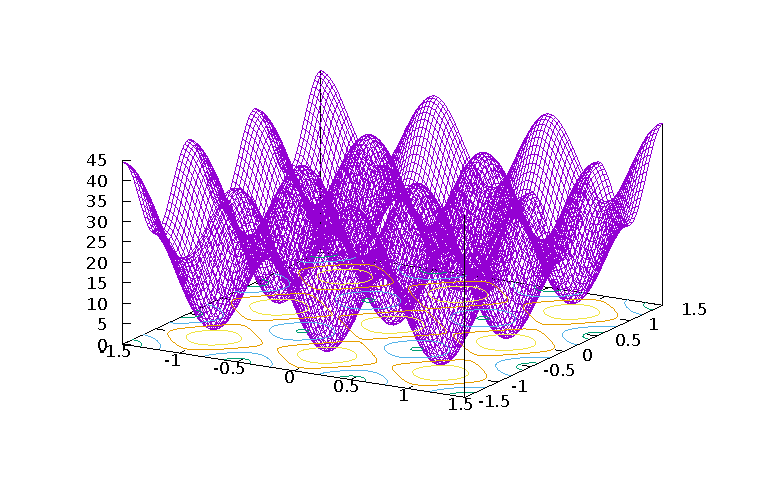
\includegraphics[width=\columnwidth]{../img/output/rastrigin}
  \caption{The Rastrigin function in three dimensions.}\label{fig:rastrigin}
\end{figure}

\begin{figure}
  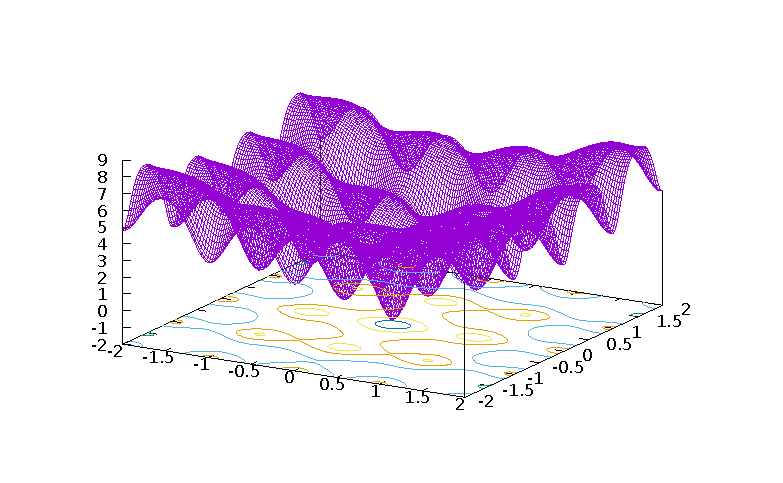
\includegraphics[width=\columnwidth]{../img/output/ackley}
  \caption{The Ackley function in three dimensions.}\label{fig:ackley}
\end{figure}


\section{Conclusion}
This paragraph will end the body of this sample document.
Remember that you might still have Acknowledgments or
Appendices; brief samples of these
follow.  There is still the Bibliography to deal with; and
we will make a disclaimer about that here: with the exception
of the reference to the \LaTeX\ book, the citations in
this paper are to articles which have nothing to
do with the present subject and are used as
examples only.
%\end{document}  % This is where a 'short' article might terminate




\bibliographystyle{ACM-Reference-Format}
\bibliography{bibliography.bib} 

\end{document}
